\documentclass[tikz,border=10pt]{standalone}
\usetikzlibrary{decorations.text}
\definecolor{econblue}{RGB}{0,61,140}
\definecolor{econgreen}{RGB}{0,132,85}
\definecolor{econred}{RGB}{184,28,45}
\definecolor{econorange}{RGB}{245,124,0}
\newcommand*{\econtextstyle}{\sffamily\large\bfseries\color{black!90}}
\newcommand{\econarcarrow}[4]{%
   % inner radius, middle radius, outer radius, start angle,
   % end angle, tip protusion angle, options, text, color
   \pgfmathsetmacro{\rin}{1.75}
   \pgfmathsetmacro{\rmid}{2.25}
   \pgfmathsetmacro{\rout}{2.75}
   \pgfmathsetmacro{\astart}{#1}
   \pgfmathsetmacro{\aend}{#2}
   \pgfmathsetmacro{\atip}{6}
   \fill[#4, very thick] (\astart+\atip:\rin)
                         arc (\astart+\atip:\aend:\rin)
      -- (\aend-\atip:\rmid)
      -- (\aend:\rout)   arc (\aend:\astart+\atip:\rout)
      -- (\astart:\rmid) -- cycle;
   \path[
      decoration = {
         text along path,
         text = {|\econtextstyle|#3},
         text align = {align = center},
         raise = -1.3ex
      },
      decorate
   ](\astart+\atip:\rmid) arc (\astart+\atip:\aend+\atip:\rmid);
}
\begin{document}
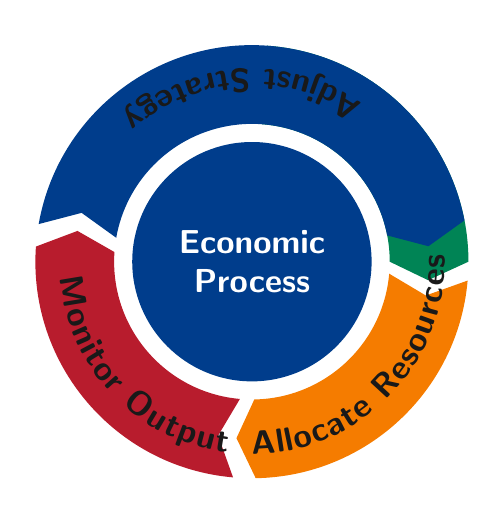
\begin{tikzpicture}
   \fill[even odd rule,econblue] circle (1.52);

   \node at (0,0) [
      font  = \econtextstyle,
      color = white,
      align = center
   ]{
      Economic\\
      Process
   };
   \econarcarrow{ 80}{  0}{ Analyze Market }{econgreen}
   \econarcarrow{265}{355}{ Allocate Resources }{econorange}
   \econarcarrow{170}{265}{ Monitor Output }{econred}
   \econarcarrow{ 5}{170}{ Adjust Strategy }{econblue}
\end{tikzpicture}
\end{document}